\section{Web Spam Detection}

\begin{frame}{Web Spam}

What constitutes web spam?

\begin{itemize}

\item auto-generated web pages that contain:

\begin{itemize}
	\item common search keywords and phrases
	\item "borrowed" content from many different pages
	\item advertisements
\end{itemize}

\item produce ad revenue by attracting traffic

\item little or no informative value to the user

\end{itemize}

What we want - detect and eliminate web spam from search results
\end{frame}

\begin{frame}{Quilted Pages}

"Quilted" page:
\begin{itemize}
	\item page made up of content borrowed from other web pages
	\item content usually comes from other domains
\end{itemize}

\begin{quote}
	Warning! Not all quilted pages are web spam.
	% blog front pages, news portals, lyrics sites, ...
\end{quote}

Using an algorithm that detects \textbf{all} quilted pages:
\begin{itemize}

\item quilt parameters:
\begin{itemize}
	\item number of sources for the content
	\item size of shingles taken into account
	\item eliminating common shingles
\end{itemize}

\item final result: only 34\% of the quilted pages were spam 
% your algorithm is bad, and you should feel bad

\item possible improvements:
\begin{itemize}
	\item semantic analysis of page content
	\item recognition by other features of web spam pages
\end{itemize}

\end{itemize}

\end{frame}

\begin{frame}{Spam Analysis (1)}
Prevalent features of web spam:
\begin{itemize}
	\item large number of words per page - keyword stuffing
	\item long words - "freedownloads", "hotelbookings"
	\item lots of \textbf{anchor words}
	\item many words in title - for SEO % grafic 1
	\item high compression ratio - redundancy due to repeated words % grafic 2
	\item low fraction of visible content - hidden tag words  % grafic 3
	\item small number of stop words % grafic 4
	% sunt clare astea? ar mai merge explicitate
\end{itemize}
\end{frame}

\begin{frame}[plain]
\begin{figure}
\centering

% 	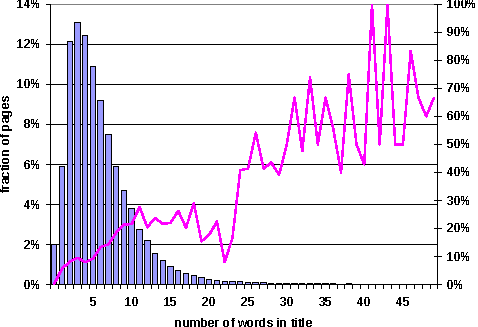
\includegraphics[width=0.5\textwidth]{img/webspam-title.pdf}
% 	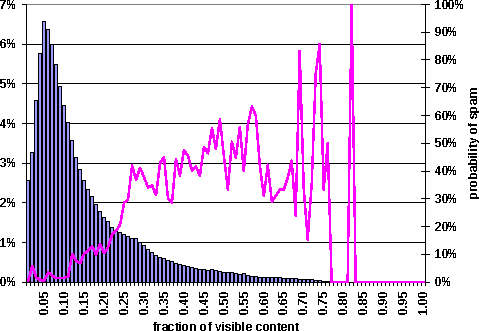
\includegraphics[width=0.5\textwidth]{img/webspam-visible.pdf}
%	\newline
% 	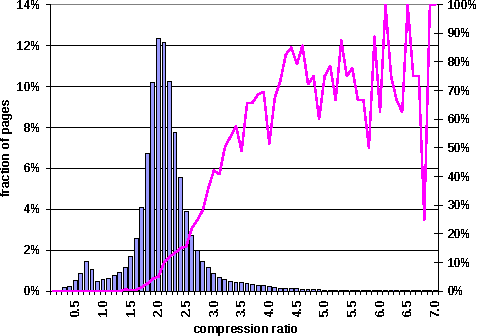
\includegraphics[width=0.5\textwidth]{img/webspam-compression.pdf}
% 	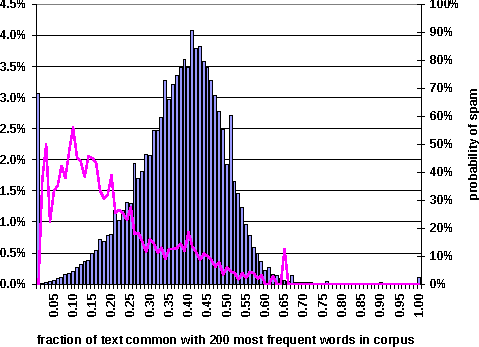
\includegraphics[width=0.5\textwidth]{img/webspam-stopwords.pdf}

 	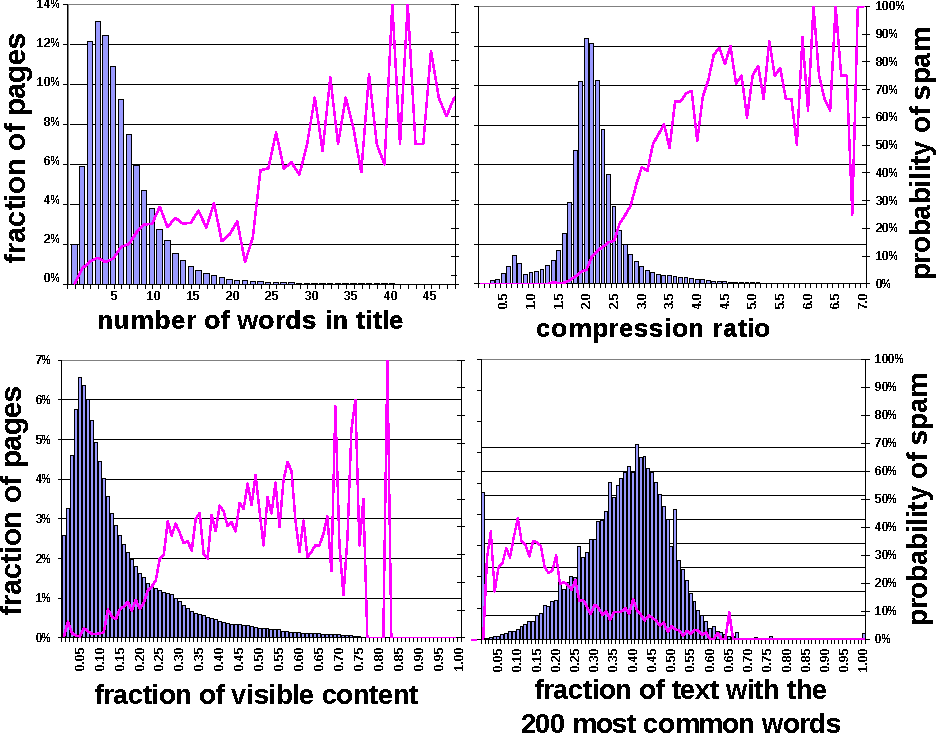
\includegraphics[width=\textwidth]{img/webspam-all.pdf}
\end{figure}
\end{frame}

\begin{frame}{Spam Analysis (3)}
\begin{columns}
	\begin{column}[r]{0.6\textwidth}
	How do we use these features?
	\begin{itemize}
	\item compute numeric ranges for each feature
	\item build a \textbf{decision tree}-based classifier
	\end{itemize}
	\end{column}

	\begin{column}[l]{0.5\textwidth}
		\begin{figure}
		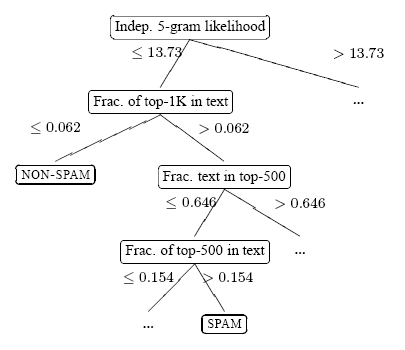
\includegraphics[width=\textwidth]{img/dtree.png}
		\end{figure}
	\end{column}
\end{columns}

Results:
\begin{itemize}
	\item spam: 91.1\% precision, 86.2\% recall
	\item non-spam: 98.7\% precision, 97.8\% recall
\end{itemize}
\end{frame}
